\documentclass[11pt]{article}
\usepackage{graphics,epsfig,amsmath,amssymb}
\usepackage{epsf}
\usepackage{boxedminipage}
\usepackage{fullpage}
\usepackage{fancyheadings}
\usepackage{times}
\usepackage{amsmath}
\usepackage{ifthen}
%\usepackage{pseudocode}
\usepackage{psfrag}
\pagestyle{fancy}

\setlength{\topmargin}{.2in}
\setlength{\parindent}{0in}
\setlength{\parskip}{.15in}
\setlength{\footskip}{0.1in}

\newcounter{pctr}
\stepcounter{pctr}

\newcounter{partctr}

\newcommand{\ie}{{\em i.e.}}
\newcommand{\eg}{{\em e.g.}}

\newcommand{\ch}{\item {\bf True~~/~~False~~}}
\newcommand{\tfnote}{\probnote{Circle True or False for each choice.}}
\newcommand{\allapply}{\probnote{Circle ALL that apply}}
\newcommand{\bestanswer}{\probnote{Circle the BEST answer}}
\newcommand{\ansbelow}{\probnote{Answer legibly in the space below.}}

\renewcommand{\thesection}{{\bf\Roman{section}}}
\renewcommand{\theenumi}{{\bf\Alph{enumi}.}}
\renewcommand{\labelenumi}{{\bf\Alph{enumi}.}}

\newcommand{\setversion}[1]{\def\version{#1}}
\setversion{quiz}

\ifthenelse{\equal{\version}{answers}}{
    \newcommand{\sols}[1]{#1}
} {
    \newcommand{\sols}[1]{}
}


\newcounter{answer}
\newenvironment{answer}[1][\relax]{\refstepcounter{answer}\begin{list}%
 {}{\leftmargin 0pt\rightmargin 0pt\labelsep 3pt\parsep 0pt%
 \setlength{\listparindent}{\parindent}}
    \item {\bf Answer \theanswer #1}\
    }{\hspace*{\fill}$\blacksquare$\end{list}} 



% uses these macros to delimit problems
\newcommand\prob[1]%
  {\begin{itemize}\item[]%
   \vspace{.2in}{\bf\thepctr. ~[#1~ points]:}\stepcounter{pctr}}
\newcommand\eprob{\end{itemize}}
\newcommand\probnote[1]%
  {\\\begin{tabular}{cr} \hspace{3in} & {\bf (#1)} \\ \end{tabular}}

% headers/footers
\lhead[\fancyplain{}{\bf Page \thepage ~of \pageref{lastpage}}]%
      {CS 6250 Fall 2010, Quiz 1}
\lfoot[{\bf Initials: }]%
      {{\bf Initials: }}
\rhead[CS 6250 Fall 2010, Quiz 1]%
      {\fancyplain{}{\bf Page \thepage ~of \pageref{lastpage}}}
\cfoot{}
\setlength{\headrulewidth}{0in}
\setlength{\headsep}{.3in}

 % Compact itemize and enumerate.  Note that they use the same counters and
% symbols as the usual itemize and enumerate environments.
\def\compactify{\itemsep=0pt \topsep=0pt \partopsep=0pt \parsep=0pt}
\let\latexusecounter=\usecounter
\newenvironment{CompactItemize}
  {\def\usecounter{\compactify\latexusecounter}
   \begin{itemize}}
  {\end{itemize}\let\usecounter=\latexusecounter}
\newenvironment{CompactEnumerate}
  {\def\usecounter{\compactify\latexusecounter}
   \begin{enumerate}}
  {\end{enumerate}\let\usecounter=\latexusecounter}

\begin{document}
\cfoot{}
\pagestyle{empty}
\begin{center}
\begin{tabular}{lr}
\resizebox{1in}{!}{
\includegraphics{GT}}
&
\parbox{4in}{
    {\Large\it College of Computing} \\ \\
    {\LARGE\sf Georgia Institute of Technology} 
}
%
\end{tabular}
\end{center}

\begin{center}
{\Large{\bf CS 6250: Computer Networking: Fall 2010} \\
 \vspace{.15in} \Huge{\bf Quiz I}} 
\vspace{.2in}

% this is the box on the first page with overall quiz information
\begin{boxedminipage}[h]{6in}
There are \underline{14 questions} and
  \underline{\pageref{lastpage} pages} in this quiz booklet (including
  this page).  Answer each question according to the instructions given.
  You have {\bf 85 minutes} to answer the questions.

%\vspace{.1in} The last page is an easy question.  {\em Rip this
%page off of your exam for five bonus points.}  Turn it in anonymously if
%you like.


\vspace{.1in} 
If you find a question ambiguous, write down any
assumptions you make.  {\bf Be neat and legible.}  If I can't
understand your answer, I can't give you credit!  There are three pretty
challenging questions (clearly marked); you may want to look through the
whole quiz and save those for last.

\vspace{.1in} 
Use the empty sides of this booklet if you need scratch space.  You
may also use them for answers, although you shouldn't need to.  {\em If you
do use the blank sides for answers, make sure to clearly say so!}

\vspace{.1in} 
{\bf Note well: Write your name in the space below AND your initials at the bottom of each
page of this booklet.}

\begin{center}{\bf THIS IS AN ``OPEN NOTES, OPEN PAPERS'' QUIZ.\\
NO OTHER MATERIALS, NO PHONES, NO COMPUTERS, NO LAPTOPS, NO PDAS.\\
%NO ENCRYPTED WIRELESS TRAFFIC. \\
MAKE SURE YOU'VE READ ALL THE INSTRUCTIONS ABOVE!}
\end{center}
{\em Initial here to indicate that (1)~you've read the instructions and (2)~
you agree to abide by the Georgia Tech Honor Code: }



\vspace{.05in} The last page has easy bonus questions, {\em which you can
answer outside of the allotted time}.  Rip the last page off of your
quiz for five bonus points.  Turn it in anonymously if you like (feel
free to fill it out after the quiz and give it to a TA, or take it with you).  You
won't get the five points if you don't tear off the page (this is to
make certain you've read this far ;).

\end{boxedminipage}
\end{center}
\vspace*{0.15in}
\begin{center}
{\it Do not write in the boxes below}
\end{center}

\begin{center}
\begin{tabular}{|l|l|l|l|l|l|l|l|l|} \hline \hline
{\bf 1-5 (xx/20)}& {\bf 6-10 (xx/27)}& {\bf 11-13 (xx/9)} &{\bf Bonus (xx+5/14)} & {\bf Total
  (xx/70)}  \\ \hline 
 & & & & \\ 
 & & & &\\ \hline \hline
\end{tabular}
\end{center}

\vspace{.1in}
{\bf\Large{Name:}}

\newpage
\pagestyle{fancy}

\section{Warmup}



\prob{4} Which of the following is true about virtual LANs?
\allapply

\setcounter{partctr}{0}
\begin{list}{\bf\Alph{partctr}.}{\usecounter{partctr}}
\item When a host sends an ARP query for some IP address, a host
  on a different virtual LAN with that IP address will not hear the
  ARP query.
\item Two hosts on different virtual LANs cannot communicate with one
  another without sending traffic through a layer 3 device (such as a router).
\item A switch port can only be trunked to a single VLAN.
\item If two wireless access points are trunked to the same VLAN, a host
  can move from one access point to another without breaking existing
  TCP connections.
\item All of the above.
\end{list}
\eprob

\sols{
\begin{answer}
The answer is: (A), (B), (D).
\end{answer}
}


\prob{4} Which of the following are true about the BGP route selection process?
\allapply

\setcounter{partctr}{0}
\begin{list}{\bf\Alph{partctr}.}{\usecounter{partctr}}
\item Local preference can be used to exercise control over inbound traffic.
\item AS path prepending can be used to exercise control over inbond
  traffic.
\item IP prefix deaggregation can be used to exercise control over
  inbound traffic.
\item When a BGP route is advertised from one AS to a neighboring AS,
  the local preference attribute is preserved.
\item None of the above.
\end{list}
\eprob

\sols{
\begin{answer}
The answer is : (B), (C).
\end{answer}
}

\prob{4} Which of the following is true about IPv4 address space exhaustion?
\allapply
\setcounter{partctr}{0}
\begin{list}{\bf\Alph{partctr}.}{\usecounter{partctr}}
%\begin{enumerate}
\item The increase in IPv4 prefixes may slow the process of IP address
  lookup. 
\item The increase in ASes that are multihomed has contributed to
  address space exhaustion.
\item Reassigning a contiguous block of IP addresses to each AS on the
  Internet could help reduce IPv4 address space exhaustion.
\item IPv4 address space exhaustion is primarily caused by the increase
  in the number of devices connected to the Internet.
\item All of the above.
\end{list}
\eprob

\sols{
\begin{answer}
The answer is: (A), (B), (C).
\end{answer}
}

\pagebreak
\prob{4} Which of the following most accurately describes the
differences between packet-level monitoring and flow-level monitoring?
\allapply
\setcounter{partctr}{0}
\begin{list}{\bf\Alph{partctr}.}{\usecounter{partctr}}
\item A network operator can determine how much each application uses
  to total traffic volume from flow-level monitoring alone.
\item A network operator can determine statistics such as the average
  delay or jitter experienced by a flow from flow-level monitoring
  alone.
%\item ISPs use packet-level monitoring as the basis for billing.
\item Trajectory sampling increases the likelihood that {\em some}
  router in the network samples traffic from a particular flow.
\item Flow statistics that are generated based on sampled packet traces
  may not have information about every flow.
\item All of the above.
\end{list}
\eprob

\sols{
\begin{answer}
The answer is (A), (D).
\end{answer}
}


\prob{4} What are some of the motivations for using a layer two topology
in a data center?
\allapply
\setcounter{partctr}{0}
\begin{list}{\bf\Alph{partctr}.}{\usecounter{partctr}}
%\begin{enumerate}
\item Layer two topologies are easier to configure than layer three topologies.
\item Layer two's ``flat'' addressing model makes it relatively easy to
  configure and perform various network operations tasks (e.g., perform
  migration). 
\item It is easier to isolate different administrative groups from one
  another on a single, flat layer two topology than it is in a topology
  with routing.
\item Spanning trees provide better robustness and load-balancing
  capabilities than IP routing protocols.
\item None of the above
\end{list}
\eprob

\sols{
\begin{answer}
The answer is (A), (B).
\end{answer}
}


%%%%%%%%%%%%%%%%%%%%%%%%%%%%%%%%%%%%%%%%%%%%%%%%%%%%%%%%%%%%

\newpage
\section{Potpourri}


\prob{5} Define the {\em end-to-end argument}.  Explain how TCP
congestion control abides by the end-to-end argument; explain the
potential drawbacks of individual routers enforcing congestion control
at each hop.~\ansbelow
\vspace{1.65in}
\eprob

\sols{
\vspace{-1.25in}
\begin{answer}
The end-to-end argument says that the ``intelligence'' for network
functions (e.g., failure recovery, in-order delivery, encryption) should
be placed at network endpoints, not at nodes in the middle of the
network.  One rationale for this argument is that, if functions are
implemented inside the network, then functions may be unnecessarily
duplicated at each network hop.

For example, hop-by-hop congestion control may unnecessarily relieve
congestion at a hop along the path that is not the path's bottleneck.
Additionally, if each hop performs congestion control, end hosts may not
know to reduce their sending rates.
\end{answer}
}

\prob{4} Network operators use virtual LANs (VLANs) to divide a single,
flat layer two topology into many distinct domains, thus limiting the
scope of broadcast traffic (e.g., ARP queries).  Several data center
topologies that we read about (e.g., SEATTLE, Portland) instead use
lookup services to limit the scope of this type of traffic.  Do layer
two architectures like SEATTLE and Portland eliminate the need for VLANs
in data centers?  Why or why not?~\ansbelow
\vspace{1.25in}
\eprob

\sols{
\vspace{-1.25in}
\begin{answer}
These layer two architectures do not necessarily eliminate the need for
VLANs in data centers.  In addition to reducing the extent and size of
each individual broadcast domain, VLANs can be used to separate
administrative domains for reasons such as security (e.g., to force all
traffic through a layer-3 firewall) or quality of service (e.g., to give
higher priority to one administrative group over another).
\end{answer}
}

\newpage

%% \prob{4} Recall from Problem Set 1 that you measured how often the OSPF
%% process sent ``Hello'' messages on each link in the topology.  (a)~What
%% is the purpose of the ``Hello'' message? (b)~The frequency of these
%% messages can be configured with a timer.  What are the advantages and
%% disadvantages of having a timer with a very small value (i.e., sending
%% very frequent ``Hello'' messages)?
%% ~\ansbelow
%% \vspace{1.25in}
%% \eprob

%% \sols{
%% \vspace{-1.25in}
%% \begin{answer}
%% \vspace{1.25in}
%% \end{answer}
%% }


%% \pagebreak
\prob{6} In Problem Set~1, you used the Click modular router to
implement a learning switch.  In this problem, you will use Click
elements to rate-limit HTTP traffic.  To do this problem, you will need
two new elements, described below:
\begin{itemize}
\item {\tt Classifier}: This element takes {\em one input} and can have
  {\em n outputs}.  Processing is {\em push}.  The
  input is {\em offset/pattern}, where the offset is in bytes.  For
  example, 
\begin{quote}
Classifier(12/0800,
             -);
\end{quote}
sends IP packets to output 1, and all other packets to output 2.  (You
can add more patterns to this list, but you will only need two outputs
for this question.)
\item {\tt Shaper}: This element ``shapes'' traffic to a maximum rate.
  It takes one parameter, {\em rate}, which is the number of packets per
  second to shape the traffic to. This element's processing is {\em
    pull}. 
\end{itemize}
(1)~Draw a Click element pipeline that takes traffic from an interface,
    {\tt eth0}, shapes traffic {\em destined for the HTTP port} to a
    maximum of 1000 packets per second, and sends the rest of traffic
    unshaped; send your output to an interface {\tt eth1}; we have
    started the pipeline for you in a diagram below; (2)~Write the Click
    configuration corresponding to this pipeline.  {\em Hint:} The
    destination port offset is 42 bytes from the beginning of the
    Ethernet frame, and port 80 is HTTP traffic.~\ansbelow
\eprob

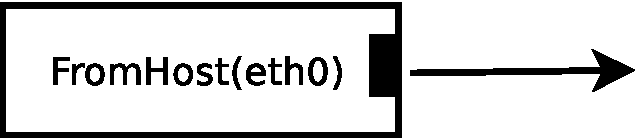
\includegraphics[width=0.3\linewidth]{click}

\vspace{1.25in}

\sols{
\begin{answer}
%\begin{verbatim}
%\end{verbatim}
\\
in :: FromHost(eth0) \\
classifier :: Classifier(42/80, -) \\
in $\rightarrow$ classifier \\
classifier[0] $\rightarrow$ Queue $\rightarrow$ Shaper(1000) $\rightarrow$ ToHost(eth0) \\
classifier[1] $\rightarrow$ ToHost(eth1)


\vspace{0.1in}
[2 points for correctly drawing the diagram; 4 points for Click
  configuration.  Partial credit for connecting elements in the right
  order.  One point for recognizing that a Queue element is needed to
  connect a push element to a pull element.]
\end{answer}
}


%% \prob{4} Recall from the {\em NetPrints} paper that the system uses the
%% notion of a ``change tree'' to help users fix their network
%% configurations.  Explain how the system constructs a change tree and the
%% relationship of a change tree to a decision tree.
%% Explain one possible case where the change tree might cause a user to make
%% an inconvenient (or incorrect) change to their home network
%% configuration. ~\ansbelow
\pagebreak
\prob{4} Explain the roles of the four ``D''s of the 4D network
architecture: What is the function of each of the the (a)~decision;
(b)~dissemination; (c)~discovery; (d)~data planes?  Explain how the
IRSCP implements each of these four ``planes''.  (Your answer should be
roughly of the form: ``The data plane [insert function here]; the
IRSCP's data plane is implemented [roughly explain how].''
\vspace{1.75in}
\eprob

\sols{
\vspace{-1.25in}
\begin{answer}
The decision plane is the ``brains'' of the network.  It effectively
takes information such as the network topology and other parameters and
sets forwarding table entries in the routers to control the forwarding
behavior of the network devices.  In the IRSCP, the decision plane is
instantiated by a route control server that collects routing information
and makes routing decisions to achieve some high-level policy.  The
dissemination plane transfers information from the routers to the
decision plane---in the case of the IRSCP, iBGP serves as the
dissemination plane.  The discovery plane allows the decision plane to
learn about information such as the network topology---in the IRSCP, the
IGP is the decision plane.  The data plane forwards traffic; the IRSCP's
data plane is implemented with routers that forward IP traffic according
to the BGP routes that the decision plane installs.
\end{answer}
}


\prob{8} 
Given the lookup table below {\em for four-bit addresses}:

\begin{center}
\begin{tabular}{|l|}
\hline
0* \\
01* \\
10* \\
101* \\
1011 \\
\hline
\end{tabular}
\end{center}
\noindent
produce the following: 
\setcounter{partctr}{0}
\begin{list}{\bf\Alph{partctr}.}{\usecounter{partctr}}
\item A two-level trie that resolves two bits at each level.
\item A four-level trie that resolves one bits at each level.
\item 
Suppose that SRAM lookup speeds are 10 nanoseconds per lookup (i.e., one
lookup takes 1 $\times 10^{-8}$ seconds).  How many packets per second
can this router forward, for each type of trie?
%
\item Assuming 1500-byte packets and 10-nanosecond lookup speeds, at
  what rate can the router forward traffic, for each type of trie.
\end{list}

~\ansbelow 
\eprob

\sols{
\begin{answer}
\begin{center}
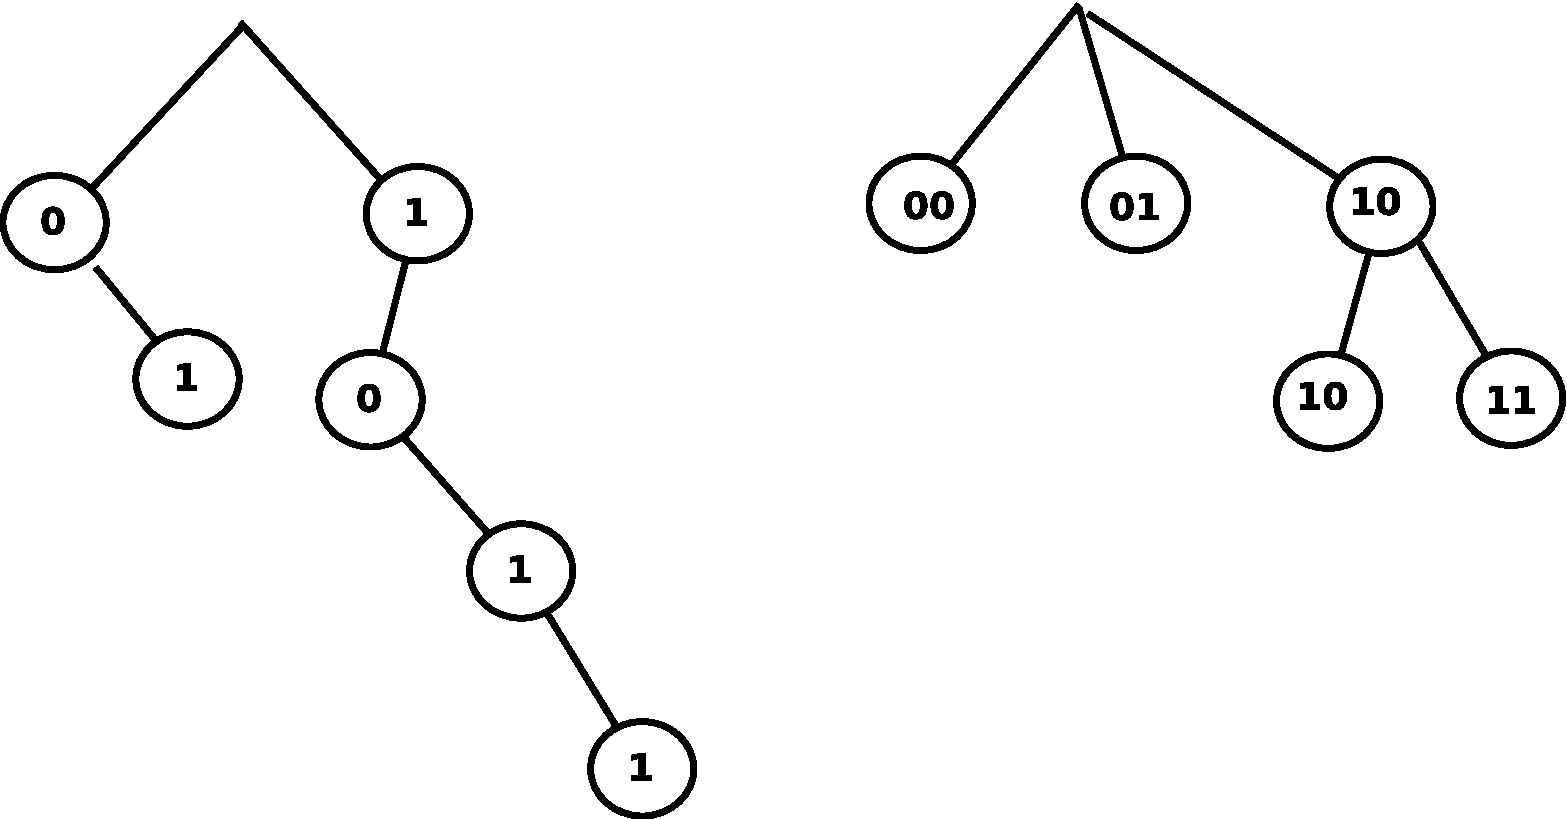
\includegraphics[width=0.75\linewidth]{tries}
\end{center}
The two-level trie would take two memory accesses to find a prefix
match (20~ns); the four-level trie would take four (40~ns).  So, the
first trie would forward (on average) one packet every $2 \times
10^{-8}$ seconds, translating to $5 \times 10^7$ packets per second.
This translates to $1500$ bytes times $8$ bits times $5 \times 10^7
\approx 600$ Gigabits per second. \\
\\
The four-level trie would forward packets only half as fast on average,
translating to $2.5\times 10^8$ packets per second, or about $300$
Gigabits per second. \\
\\
{\em Two points for drawing each trie correctly.  Three points for part (c),
  and one point for part (d).}
\end{answer}
}

\newpage
\section{Design Question: Interdomain Routing}

Consider the BGP routing table below:

\begin{small}
\begin{verbatim}
*  12.148.128.0/23  154.11.11.113            0      0      0 852 174 7018 2386 i
*  12.148.128.0/23  154.11.98.225            0      0      0 852 174 7018 2386 i
*  12.148.128.0/23  147.28.7.2               0      0      0 3130 1239 7018 2386 i
*  12.148.128.0/23  12.0.1.63                0      0      0 7018 2386 i
\end{verbatim}
\end{small}

\prob{3} Circle which route this router would select for {\tt
  143.215.129.92}; which route selection criterion would this router use
to ``break ties'' between the multiple routing choices in the table above.
~\ansbelow
\eprob

\sols{
\begin{answer}
The router would select the last route in the routing table, because the
AS path is the shortest (assume that local preference values are the
same for each of these routes).  The selection criterion that the router
would use to break ties is ``shortest AS path'' (the second stage of the
route selection process).
\vspace{0.1in}
[1 point for circling the best route; 2 points for identifying the
  correct step in the route selection process.]
\end{answer}
}


\prob{3} What is the next-hop IP address for the route that you have
  selected above?  How would this router determine the outgoing
  interface corresponding to that IP address?
~\ansbelow
\vspace{1.25in}
\eprob

\sols{
\vspace{-1in}
\begin{answer}
The next-hop IP address is {\tt 12.0.1.63}.  The router might learn
this IP address in a number of ways, including a static route or dynamic
routing (e.g., an IGP such as OSPF).  

\vspace{0.1in}
[1 point for identifying the next-hop IP address; 2 points for
  explaining how that IP address is reachable.]

\end{answer}
}

\pagebreak
\prob{3} Notice that the routing table has two different BGP routes
  with the same next-hop AS.  What is the next-hop AS?  Why might that
  AS have advertise two routes with the same AS path to this router?
~\ansbelow
\vspace{1.25in}
\eprob

\sols{
\vspace{-1in}
\begin{answer}
The next-hop AS is 852.  That AS might advertise two routes to this
router for any of the reasons related to the benefits of multihoming
(e.g., availability, reliability, performance, load balance).

\vspace{0.1in}
[1 point for identifying the next-hop AS; 2 points for explaining
  multihoming as the reason why you might see two routes appear from the
  same next-hope AS.]
\end{answer}
}

\prob{9} {\em Bonus.}
George Burdell observes that IP routing tables have grown excessively
over the last several years, and that one of the causes is that prefixes
must fall on power of two boundaries: ``If each IP address range could
be an {\em arbitrary} range, instead of falling on power-of-two
boundaries, much less IP address space would be wasted.''

\setcounter{partctr}{0}
\begin{list}{\bf\Alph{partctr}.}{\usecounter{partctr}}
\item How would you test George's hypothesis?  (Hint: think about how you
  might scalably ``probe'' to determine whether addresses in the
  Internet's routing table were actually being used)
\item Sketch a rough design/approach for how you might execute a
  ``smallest range'' match for IP address ranges that are not a power of
  two.  (Your solution need not be efficient, but it should be correct!
  {\em Hint:} Also remember that you might have overlapping prefixes
  that are not strict subsets of one another.)
\end{list}
~\ansbelow
\eprob

\sols{
\begin{answer}
There are many plausible answers to this question.  One plausible way to
do this would be to create a {\em range} for each routing table address,
and search the routing table entries for any matching entries.  One
could then pick the matching entry with the shortest range. There could
be many possible ways to do this; one possibility might be to construct
a B-tree (as is done with database indexes of this kind).
\end{answer}
}


\newpage
\section{Bonus: Anonymous Course Feedback}

{\bf This page is anonymous.}  Rip this off from your exam, and turn it
in separately if you like.  You'll get five points for simply ripping
off the last page of the exam, but I'd prefer if you fill it out and
hand it in in a separate stack.
\vspace{.5in}

What are the things you like most about the course so far?  Anything is
fair game here (topics, course structure, board technique, etc.).
\vspace{1.5in}


What are the things you like least about the course so far?  Again,
anything is fair game.
\vspace{1in}


What topics would you like to see covered?
\vspace{1in}



\label{lastpage}
\end{document}
